\documentclass{article}

\usepackage[T1]{fontenc}
\usepackage{textcomp}

\usepackage[english]{babel}
\usepackage[utf8]{inputenc}

\usepackage{lmodern}

\usepackage{hyperref}
\hypersetup{breaklinks}
\hypersetup{pdfborder=0 0 0}

\usepackage[babel=true]{microtype}

\usepackage{amsmath}

\usepackage{geometry}

\usepackage{tikz}

\usepackage[normalem]{ulem}


\title{The impact of vector interaction with other insect species on
  disease spread}

\author{
  Elizabeth Borer
  \and
  David Crowder
  \and
  Deborah Finke
  \and
  Jing Li
  \and
  Jan Medlock
  \and
  David Pattemore
  \and
  Rakefet Sharon
}


\newcommand{\md}{\mathrm{d}}
\newcommand{\me}{\mathrm{e}}
\newcommand{\mat}[1]{\mathbf{#1}}
\renewcommand{\vec}[1]{\mathbf{#1}}

\newcommand{\comment}[1]{\textbf{#1}}


\begin{document}

\maketitle

\section{Model}

Let $P_s(t)$ and $P_i(t)$ be the number of susceptible and infected
plants at time $t$.  Let $V_{sm}(t)$ be the number of susceptible
vectors moving, $V_{sfs}(t)$ be the number of susceptible vectors
feeding on susceptible plants, $V_{sfip}(t)$ be the number of
susceptible vectors feeding on infectious plants prior to being able
to acquire the pathogen, and $V_{sfit}(t)$ be the number of
susceptible vectors that are able to acquire the virus.  Similarly,
let $V_{im}(t)$ be the number of infectious vectors moving,
$V_{ifsp}(t)$ be the number of infectious vectors feeding on
susceptible plants prior to being able to transmit the pathogen,
$V_{ifst}(t)$ be the number of infectious vectors feeding on
susceptible plants that are able to transmit the virus, and
$V_{ifi}(t)$ be the number of infectious vectors feeding on infectious
plants.  The total number of vectors is
\begin{equation}
  V = V_{sm} + V_{sfs} + V_{sfip} + V_{sfit} + V_{im} + V_{ifsp} +
  V_{ifst} + V_{ifi}
\end{equation}
and the total number of plants is
\begin{equation}
  P = P_s + P_i.
\end{equation}
The vectors feed on new plants at the rate $f_V$ and spend the
proportion $\phi_V$ of their time feeding and $1 - \phi_V$ moving.  We
assume that vectors only reproduce when they are feeding; the birth
rate is proportional to the number of the feeding vectors, with a
logistic term dependent on the total number of vectors; and the
newborns join the moving group.  Moving and feeding vectors die but at
different rates, with moving vectors assumed to die more quickly than
feeding vectors (i.e.~$\delta_V > 0$).

The model is
\begin{equation}
  \label{odesystem}
  \begin{split}
    \frac{\md V_{sm}}{\md t}
    &=
    - \underbrace{\frac{f_V}{1 - \phi_V} V_{sm}}_{\text{to feeding}}
    + \underbrace{\frac{f_V}{\phi_V} (V_{sfs} + V_{sfip} + V_{sfit})}_{\text{from feeding}}
    + \underbrace{\gamma_V V_{im}}_{\text{loses pathogen}}
    - \underbrace{(1 + \delta_V) \mu_V V_{sm}}_{\text{death}}
    \\ & \quad\quad {}
    + \underbrace{b_V V_f \left(1 - \frac{V}{K_V P}\right)}_{\text{birth}},
    \\
    \frac{\md V_{sfs}}{\md t}
    &=
    \underbrace{\frac{f_V}{1 - \phi_V} \frac{P_s}{P} V_{sm}}_{\text{from moving}}
    - \underbrace{\frac{f_V}{\phi_V} V_{sfs}}_{\text{to moving}}
    + \underbrace{\gamma_V (V_{ifsp} + V_{ifst})}_{\text{loses pathogen}}
    - \underbrace{\mu_V V_{sfs}}_{\text{death}}
    - \underbrace{\beta_P \frac{V_{ifst}}{P_s} V_{sfs}}_{\text{plant
        infected}},
    \\
    \frac{\md V_{sfip}}{\md t}
    &=
    \underbrace{\frac{f_V}{1 - \phi_V} \frac{P_i}{P} V_{sm}}_{\text{from moving}}
    - \underbrace{\frac{f_V}{\phi_V} V_{sfip}}_{\text{to moving}}
    + \underbrace{\gamma_V V_{ifi}}_{\text{loses pathogen}}
    - \underbrace{\mu_V V_{sfip}}_{\text{death}}
    + \underbrace{\beta_P \frac{V_{ifst}}{P_s} V_{sfs}}_{\text{plant infected}}
    - \underbrace{\alpha_V V_{sfip}}_{\text{acquiring}},
    \\
    \frac{\md V_{sfit}}{\md t}
    &=
    - \underbrace{\frac{f_V}{\phi_V} V_{sfit}}_{\text{to moving}}
    - \underbrace{\mu_V V_{sfit}}_{\text{death}}
    + \underbrace{\alpha_V V_{sfip}}_{\text{acquiring}}
    - \underbrace{\beta_V V_{sfit}}_{\text{infection}},
    \\
    \frac{\md V_{im}}{\md t}
    &=
    - \underbrace{\frac{f_V}{1 - \phi_V} V_{im}}_{\text{to feeding}}
    + \underbrace{\frac{f_V}{\phi_V} (V_{ifsp} + V_{ifst} + V_{ifi})}_{\text{from feeding}}
    - \underbrace{\gamma_V V_{im}}_{\text{loses pathogen}}
    - \underbrace{(1 + \delta_V) \mu_V V_{im}}_{\text{death}},
    \\
    \frac{\md V_{ifsp}}{\md t}
    &=
    \underbrace{\frac{f_V}{1 - \phi_V} \frac{P_s}{P} V_{im}}_{\text{from moving}}
    - \underbrace{\frac{f_V}{\phi_V} V_{ifsp}}_{\text{to moving}}
    - \underbrace{\gamma_V V_{ifsp}}_{\text{loses pathogen}}
    - \underbrace{\mu_V V_{ifsp}}_{\text{death}}
    - \underbrace{\beta_P \frac{V_{ifst}}{P_s} V_{ifsp}}_{\text{plant infected}}
    - \underbrace{\alpha_V V_{ifsp}}_{\text{transmitting}},
    \\
    \frac{\md V_{ifst}}{\md t}
    &=
    - \underbrace{\frac{f_V}{\phi_V} V_{ifst}}_{\text{to moving}}
    - \underbrace{\gamma_V V_{ifst}}_{\text{loses pathogen}}
    - \underbrace{\mu_V V_{ifst}}_{\text{death}}
    - \underbrace{\beta_P \frac{V_{ifst}}{P_s} V_{ifst}}_{\text{plant infected}}
    + \underbrace{\alpha_V V_{ifsp}}_{\text{transmitting}},
    \\
    \frac{\md V_{ifi}}{\md t}
    &=
    \underbrace{\frac{f_V}{1 - \phi_V} \frac{P_i}{P} V_{im}}_{\text{from moving}}
    - \underbrace{\frac{f_V}{\phi_V} V_{ifi}}_{\text{to moving}}
    - \underbrace{\gamma_V V_{ifi}}_{\text{loses pathogen}}
    - \underbrace{\mu_V V_{ifi}}_{\text{death}}
    + \underbrace{\beta_P \frac{V_{ifst}}{P_s} (V_{ifsp} + V_{ifst})}_{\text{plant infected}}
    \\ & \quad\quad {}
    + \underbrace{\beta_V V_{sfit}}_{\text{infection}},
    \\
    \frac{\md P_s}{\md t}
    &=
    - \underbrace{\beta_P V_{ifst}}_{\text{infection}},
    \\
    \frac{\md P_i}{\md t}
    &=
    \underbrace{\beta_P V_{ifst}}_{\text{infection}},
  \end{split}
\end{equation}
where the number of feeding vectors is
\begin{equation}
  V_f = V_{sfs} + V_{sfip} + V_{sfit} + V_{ifsp} + V_{ifst} + V_{ifi},
\end{equation}
$\beta_V$ is the infection rate from plants to vectors, $\beta_P$ is
the infection rate from vectors to plants, $\alpha_V$ is the rate of
vectors becoming able to acquire or transmit the pathogen, $\gamma_V$
is the rate of pathogen clearance in vectors, $\mu_V$ is the death
rate of the feeding vectors, $\delta_V$ is the proportional increase
in the death rate for moving vectors, $b_V$ is the birth rate of
vectors, and $K_V$ is the carrying capacity of vectors per plant
(\autoref{fig:full_model_diagram}).

\begin{figure}
  \centering
  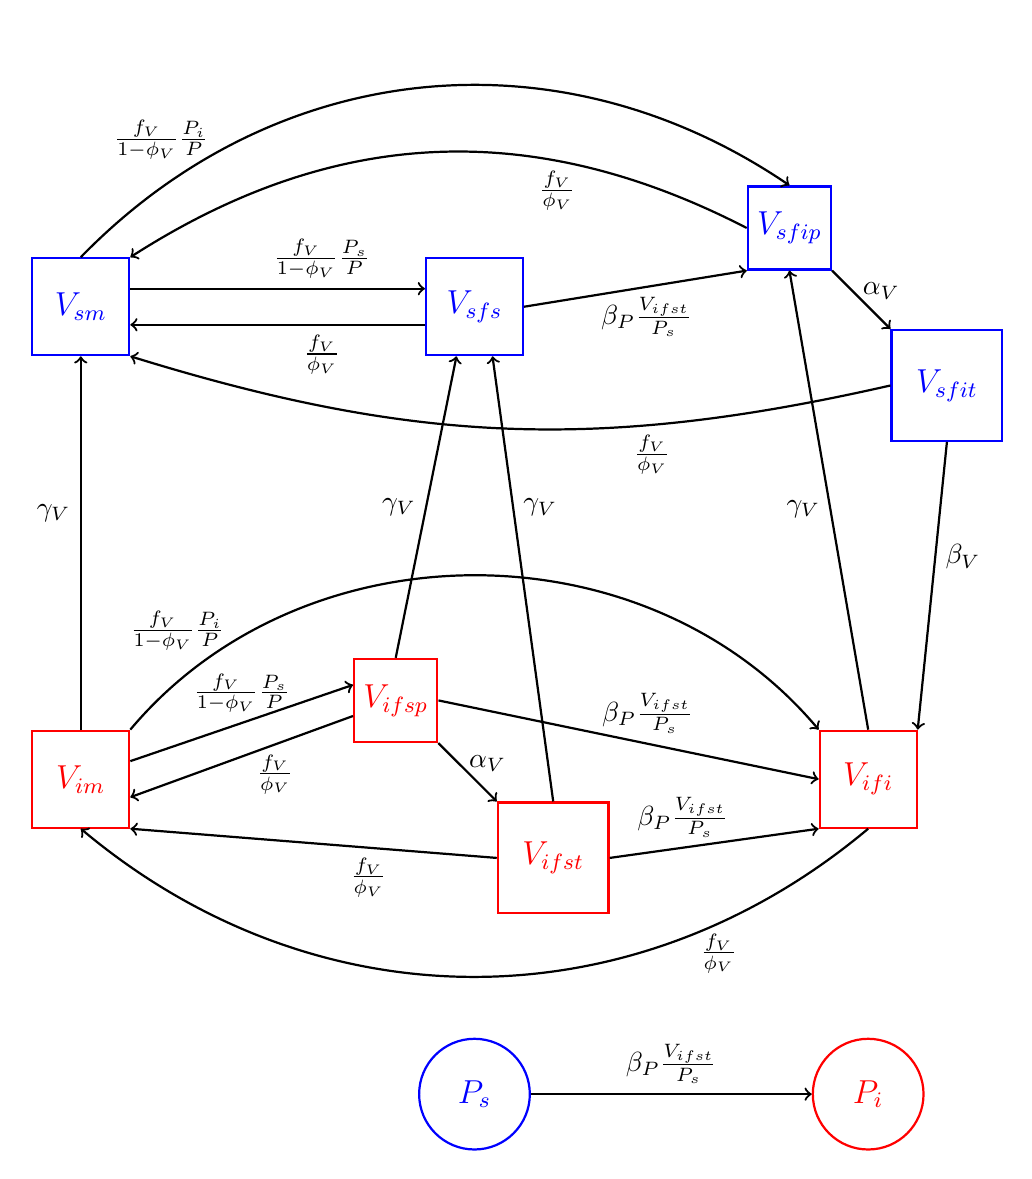
\begin{tikzpicture}[
    thick,
    scale = 1,
    compartment/.style = {draw,
      font = \large},
    plant/.style = {circle,
      minimum size = {4em}},
    susceptible/.style = {blue},
    infected/.style = {red},
    vector/.style = {rectangle,
      minimum size = {3.5em}},
    front/.style = {minimum size = {4em}},
    back/.style = {minimum size = {3em}},
    ]

    \node at (0, 10)
    [compartment, vector, susceptible, name = V_sm] {$V_{sm}$};

    \node at (5, 10)
    [compartment, vector, susceptible, name = V_sfs] {$V_{sfs}$};

    \node at (9, 11)
    [compartment, vector, susceptible, back, name = V_sfip] {$V_{sfip}$};
    \node at (11, 9)
    [compartment, vector, susceptible, front, name = V_sfit] {$V_{sfit}$};

    \node at (0, 4)
    [compartment, vector, infected, name = V_im] {$V_{im}$};

    \node at (4, 5)
    [compartment, vector, infected, back, name = V_ifsp] {$V_{ifsp}$};
    \node at (6, 3)
    [compartment, vector, infected, front, name = V_ifst] {$V_{ifst}$};

    \node at (10, 4)
    [compartment, vector, infected, name = V_ifi] {$V_{ifi}$};

    \node at (5, 0)
    [compartment, plant, susceptible, name = P_s] {$P_s$};
    \node at (10, 0)
    [compartment, plant, infected, name = P_i] {$P_i$};

    \draw [->] (P_s) to node [above] {$\beta_P \frac{V_{ifst}}{P_s}$} (P_i);

    \draw [->] (V_sfip) to node [right, pos = 0.35] {$\alpha_V$} (V_sfit);
    \draw [->] (V_ifsp) to node [right, pos = 0.35] {$\alpha_V$} (V_ifst);

    \draw [->] (V_sfit.270) to node [right, pos = 0.4] {$\beta_V$} (V_ifi.45);

    \draw [->] (V_im) to node [left, pos = 0.58] {$\gamma_V$} (V_sm);
    \draw [->] (V_ifsp.90) to node [left] {$\gamma_V$} (V_sfs.250);
    \draw [->] (V_ifst.90) to node [right, pos = 0.66] {$\gamma_V$} (V_sfs.290);
    \draw [->] (V_ifi.90) to node [left, pos = 0.48] {$\gamma_V$} (V_sfip.270);

    \draw [->] (V_sm.20) to node [above, pos = 0.65]
    {$\frac{f_V}{1 - \phi_V} \frac{P_s}{P}$} (V_sfs.160);
    \draw [->] (V_sm.90) to [bend left = 40] node
    [left, pos = 0.25, xshift = -8]
    {$\frac{f_V}{1 - \phi_V} \frac{P_i}{P}$} (V_sfip.90);

    \draw [->] (V_im.20) to node [above]
    {$\frac{f_V}{1 - \phi_V} \frac{P_s}{P}$} (V_ifsp.160);
    \draw [->] (V_im.45) to [bend left = 50] node
    [left, pos = 0.2, xshift = -6]
    {$\frac{f_V}{1 - \phi_V} \frac{P_i}{P}$} (V_ifi.135);

    \draw [->] (V_sfs.200) to node [below, pos = 0.35]
    {$\frac{f_V}{\phi_V}$} (V_sm.340);
    \draw [->] (V_sfip.180) to [bend right = 30] node [below, pos = 0.3]
    {$\frac{f_V}{\phi_V}$} (V_sm.45);
    \draw [->] (V_sfit.180) to [bend left = 15] node [below, pos = 0.3]
    {$\frac{f_V}{\phi_V}$} (V_sm.315);

    \draw [->] (V_ifsp.200) to node [below, pos = 0.35]
    {$\frac{f_V}{\phi_V}$} (V_im.340);
    \draw [->] (V_ifst.180) to node [below, pos = 0.35]
    {$\frac{f_V}{\phi_V}$} (V_im.315);
    \draw [->] (V_ifi.270) to [bend left = 40] node [below, pos = 0.2]
    {$\frac{f_V}{\phi_V}$} (V_im.270);

    \draw [->] (V_sfs.0) to node [below, pos = 0.55]
    {$\beta_P \frac{V_{ifst}}{P_s}$} (V_sfip.225);
    \draw [->] (V_ifsp.0) to node [above, pos = 0.55]
    {$\beta_P \frac{V_{ifst}}{P_s}$} (V_ifi.180);
    \draw [->] (V_ifst.0) to node [above, pos = 0.35]
    {$\beta_P \frac{V_{ifst}}{P_s}$} (V_ifi.225);

    % \draw [<-] (V_sm.110) to node [left, pos = 0.8]
    % {$b_V V_f \left(1 - \frac{V}{K_V P}\right)$} +(90: 1.5);

    % \draw [->] (V_sm.70) to node [right, pos = 0.8]
    % {$(1 + \delta_V) \mu_V$} +(90: 1.5);
    % \draw [->] (V_im) to node [right, pos = 0.8]
    % {$(1 + \delta_V) \mu_V$} +(270: 2);

    % \draw [->] (V_sfs) to node [right, pos = 0.8]
    % {$\mu_V$} +(90: 2);
    % \draw [->] (V_sfip) to node [right, pos = 0.8]
    % {$\mu_V$} +(90: 2);
    % \draw [->] (V_sfit) to node [right, pos = 0.8]
    % {$\mu_V$} +(90: 2);
    % \draw [->] (V_ifsp) to node [right, pos = 0.8]
    % {$\mu_V$} +(270: 2);
    % \draw [->] (V_ifst) to node [right, pos = 0.8]
    % {$\mu_V$} +(270: 2);
    % \draw [->] (V_ifi) to node [right, pos = 0.8]
    % {$\mu_V$} +(270: 2);
  \end{tikzpicture}
  \caption{Model diagram.  $P_s$ and $P_i$ are the numbers
    of susceptible and infectious plants.  $V_{sm}$ is the number of
    susceptible vectors moving, $V_{sfs}$ is the number of susceptible
    vectors feeding on susceptible plants, $V_{sfip}$ is the number of
    susceptible vectors feeding on infectious plants prior to being
    able to acquire the pathogen, and $V_{sfit}$ is the number of
    susceptible vectors feeding on infectious plants that are able to
    acquire the pathogen.  Similarly, $V_{im}$ is the number of
    infectious vectors moving, $V_{ifsp}$ is the number of infectious
    vectors feeding on susceptible plants prior to being able to
    transmit the pathogen, $V_{ifst}$ is the number of infectious
    vectors feeding on susceptible plants that are able to transmit the
    pathogen, and $V_{ifi}$ is the number of infectious vectors
    feeding on infectious plants.}
  \label{fig:full_model_diagram}
\end{figure}


\begin{table}
  \centering
  \begin{tabular}{llr}
    \multicolumn{2}{l}{\textbf{Parameter}}
    & \multicolumn{1}{r}{\textbf{Value}}
    \\
    $f_V$ & Plants fed on per unit time & $6\;\text{d}^{-1}$
    \\
    $\phi_V$ & Fraction of time vectors spend feeding & $0.5$
    \\
    $\mu_V$ & Mortality rate for feeding vectors & $0.02\;\text{d}^{-1}$
    \\
    $\delta_V$ & Relative mortality increase for moving vectors & $1$
    \\
    $b_V$ & Fecundity of feeding vectors & $0.08\;\text{d}^{-1}$
    \\
    $K_V$ & Carrying capacity of vectors per plant & $100$
    \\
    $V(0)$ & Initial number of vectors & $100$
    \\
    $P(0)$ & Initial number of susceptible & $10\,000$
    \\
    \multicolumn{3}{c}{\textbf{Persistent}}
    \\
    $\beta_V$ & Transmission rate from plants to vectors & $8.3\;\text{d}^{-1}$
    \\
    $\beta_P$ & Transmission rate from vectors to plants & $5.5\;\text{d}^{-1}$
    \\
    $\alpha_V$ & Rate of vectors becoming able to acquire or transmit & $48\;\text{d}^{-1}$
    \\
    $\gamma_V$ & Rate of pathogen clearance in vectors & $0\;\text{d}^{-1}$
    \\
    \multicolumn{3}{c}{\textbf{Non-persistent}}
    \\
    $\beta_V$ & Transmission rate from plants to vectors & $500\;\text{d}^{-1}$
    \\
    $\beta_P$ & Transmission rate from vectors to plants & $1\,000\;\text{d}^{-1}$
    \\
    $\alpha_V$ & Rate of vectors becoming able to acquire or transmit & $86\,400\;\text{d}^{-1}$
    \\
    $\gamma_V$ & Rate of pathogen clearance in vectors & $0.12\;\text{d}^{-1}$
  \end{tabular}
  \caption{Model parameters and initial conditions.}
  \label{params}
\end{table}


\section{Results}

\begin{itemize}
\item The pathogen grows slowly until the vector population becomes
  large (\autoref{fig:solutions}).

\item The pathogen growth rate increases as the vector population
  grows (\autoref{fig:growth_rates}).

\item The growth rate is insensitive to the feeding rate
  (\hyperref[fig:sensitivity_1param]{Figures
    \ref*{fig:sensitivity_1param}}--\ref{fig:sensitivity_2params}).
\end{itemize}


\begin{figure}
  \centering
  \includegraphics[width = \textwidth]{solutions}
  \caption{Model solutions for persistent and non-persistent
    scenarios.  Parameter values are given in \autoref{params}.
    For initial conditions, we used the result from the quasi-steady
    state approximation (\autoref{sec:QSSA}) that $50\%$ of the
    vectors are moving and $50\%$ are feeding for our parameter
    values, and that 1 of the moving vectors are infected and all
    others are uninfected ($V_{sm}(0) = 49, V_{im}(0) = 1, V_{sfs}(0) =
    50, V_{sfi}(0) = V_{ifs}(0) = V_{ifi}(0) = 0$).}
  \label{fig:solutions}
\end{figure}

\begin{figure}
  \centering
  \includegraphics[width = \textwidth]{growth_rates}
  \caption{Intrinsic growth rate of the pathogen.  Model initial
    conditions were the disease-free state given by the parameters
    (\autoref{params}) and the result from the quasi-steady state
    approximation (\autoref{sec:QSSA}) that $50\%$ of the vectors are
    moving and $50\%$ are feeding for our parameter values ($V_{sm}(0)
    = V_{sfs}(0) = 50, P_s(0) = 10\,000, V_{im}(0) = V_{sfi}(0) =
    V_{ifs}(0) = V_{ifi}(0) = P_i(0) = 0$).}
  \label{fig:growth_rates}
\end{figure}

\begin{figure}
  \centering
  \includegraphics[width = \textwidth]{sensitivity_1param}
  \caption{Intrinsic growth rate of the pathogen vs.~parameter values
    at $150~\text{d}$, relative to its value for the baseline
    parameter value.  The dotted horizontal lines show the baseline
    parameter values.  Parameter values and initial conditions are as
    in \autoref{fig:growth_rates}.}
  \label{fig:sensitivity_1param}
\end{figure}

\begin{figure}
  \centering
  \includegraphics[width = \textwidth]{sensitivity_1param_fV}
  \caption{Intrinsic growth rate of the pathogen vs.~the feeding rate
    ($f_V$) at $150~\text{d}$, relative to its value for the baseline
    parameter value.  The vertical axis has a linear scale, compared
    to a log scale in \autoref{fig:growth_rates}, to show the smaller
    differences in growth rate as feeding rate varies.  The dotted
    horizontal lines show the baseline parameter values.  Parameter
    values and initial conditions are as in
    \autoref{fig:growth_rates}.}
  \label{fig:sensitivity_1param_fV}
\end{figure}

\begin{figure}
  \centering
  \includegraphics[width = \textwidth]{sensitivity_2params}
  \caption{Intrinsic growth rate of the pathogen vs.~parameter values
    at $150~\text{d}$, relative to its value for the baseline
    parameter value.  Parameter values and
    initial conditions are as in \autoref{fig:growth_rates}.}
  \label{fig:sensitivity_2params}
\end{figure}


\clearpage
\appendix
\section{Quasi-steady-state approximation}
\label{sec:QSSA}

Under the quasi-steady-state approximation, we take the movement rate
to be fast relative to all the other rates, i.e.~$f_V \to \infty$ and
all other parameters $\operatorname{O}(1)$.  Then terms in $f_V$ from
the differential equations give
\begin{equation}
  \begin{split}
    \frac{1}{1 - \phi_V} V_{sm} &=
    \frac{1}{\phi_V} (V_{sfs} + V_{sfip} + V_{sfit}),
    \\
    \frac{1}{1 - \phi_V} \frac{P_s}{P} V_{sm} &=
    \frac{1}{\phi_V} V_{sfs},
    \\
    \frac{1}{1 - \phi_V} \frac{P_i}{P} V_{sm} &=
    \frac{1}{\phi_V} V_{sfip},
    \\
    0 &=
    \frac{1}{\phi_V} V_{sfit},
    \\
    \frac{1}{1 - \phi_V} V_{im} &=
    \frac{1}{\phi_V} (V_{ifsp} + V_{ifst} + V_{ifi}),
    \\
    \frac{1}{1 - \phi_V} \frac{P_s}{P} V_{im} &= \frac{1}{\phi_V} V_{ifsp},
    \\
    0 &= \frac{1}{\phi_V} V_{ifst},
    \\
    \frac{1}{1 - \phi_V} \frac{P_i}{P} V_{im} &= \frac{f_V}{\phi_V} V_{ifi}.
  \end{split}
\end{equation}
Thus, the QSSA is
\begin{equation}
  \begin{aligned}
    V_{sm} &= (1 - \phi_V) V_s,
    &
    V_{sfs} &= \phi_V \frac{P_s}{P} V_s,
    &
    V_{sfip} &= \phi_V \frac{P_i}{P} V_s,
    &
    V_{sfit} &= 0,
    \\
    V_{im} &= (1 - \phi_V) V_i,
    &
    V_{ifsp} &= \phi_V \frac{P_s}{P} V_i,
    &
    V_{ifst} &= 0,
    &
    V_{ifi} &= \phi_V \frac{P_i}{P} V_i,
  \end{aligned}
\end{equation}
with
\begin{equation}
  \begin{split}
    V_s &= V_{sm} + V_{sfs} + V_{sfip} + V_{sfit}, \\
    V_i &= V_{im} + V_{ifsp} + V_{ifst} + V_{ifi}.
  \end{split}
\end{equation}


\end{document}
